\header{
    \headtitle{Charlotte} \label{charlotte}
    %
    
    \insertComment{Variante de la chanson "La carotte". Toutes deux publiée en 1911.}{}
}
\vspace{-0.3cm}
\enluminure{4}{\href{https://www.youtube.com/watch?v=BKY8kfOs7_g}{D}}{ans} son boudoir la petite Charlotte
\\Chaude du con faute d'avoir un vit
\\Se masturbait avec une carotte
\\Et jouissait sur le bord de son lit
\\\\\textbf{Refrain :}
\\Branle, branle, branle Charlotte
\\Branle, branle, ça fait du bien
\\Branle, branle, branle Charlotte
\\Branle, branle, jusqu'à demain, à deux mains, à deux mains.
\\\\Ah! Disait-elle, dans le siècle où nous sommes
\\Il faut savoir se passer des garçons,
\\Moi pour ma part je me fous bien des hommes
\\Avec ardeur je me branle le con.
\\\\Alors sa main n'étant plus paresseuse
\\Allait venait comme un petit ressort
\\Et faisait jouir la petite vicieuse
\\Aussi ce jeu lui plaisait-il bien fort.
\\\\Mais ô malheur, ô fatale disgrâce
\\Dans son bonheur elle fit un brusque saut
\\Du contrecoup la carotte se casse
\\Et dans le con il en reste un morceau.
\\\\Un médecin praticien fort habile
\\Fut appelé qui lui fit bien du mal
\\Mais par malheur la carotte indocile
\\Ne put sortir du conduit vaginal.
\\\\Mesdemoiselles que le sort de Charlotte
\\Puisse longtemps vous servir de leçon
\\Ah, croyez moi, laissez là la carotte
\\Préférez lui le vit d'un beau garçon
\breakpage
\textbf{Refrain final :}
\\Baise, Baise, Baise Charlotte
\\Baise, Baise, ça fait du bien
\\Baise, Baise, Baise Charlotte
\\Baise, Baise, jusqu'à demain
\\A deux mains, à deux mains
\\
\begin{center}
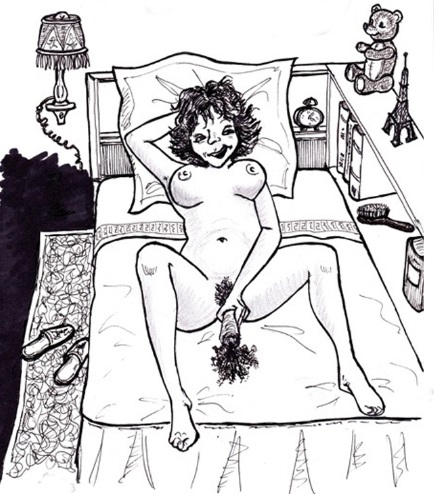
\includegraphics[width=1\textwidth]{images/charlotte.jpg}
\end{center}

\breakpage